
\section{Dwi Yulianingsih}
\subsection{Sejarah Phyton}
Phyton adalah sebuah bahasa pemrograman dengan perancangan yang berfokus pada tingkat keterbacaan kode, menggabungkan kapabilitas, kemampuan dan sintaks kode yang sangat jelas. Phyton juga dilengkapi dengan fungsi pustaka atau library standar yang besar dan didukung oleh komunitas yang besar. Phyton dibuat oleh seseorang keturunan belanda yaitu Guido Van Rossum, awalnya pembuatan phyton ini digunakan untuk pembuatan bahasa tingkat tinggi pada sebuah sistem operasi. Phyton telah digunakan oleh perusahaan-perusahaan untuk membuat perangkat lunak komersil. Pemrograman bahasa python merupakan pemrogram gratis atau freeware, sehingga bisa dikembangkan, dan tidak memiliki batasan dalam peng-copy-an dan didistribusikan. Terdapat beberapa layanan yang diberikan dalam phyton lengkap dengan source kodenya, debugger dan profiler, antarmuka, fungsi sistem, GUI, dan database-nya. Python dapat digunakan untuk berbagai Sistem Operasi, yang diantaranya Unix (linux), PCs (DOS, Windows, OS/2), Machintosh dan sebagainya.

\subsection{Instalasi Anaconda}
\begin{enumerate}
    \item Kita harus menyiapkan instalasi anaconda, kita dapat mendownload nya melalui internet.
    \item Kemudian kita bisa mengklik installer yang telah kita miliki dan tunggu.
    \begin{figure}[!htbp]
        \centering
        \includegraphics[width=3cm,height=3cm]{figures/1.png}
        \caption{gambar1}
        \label{awal}
        \end{figure}

    \item Lalu pada tampilan seperti gambar di bawah klik next.
    \begin{figure}[!htbp]
        \centering
        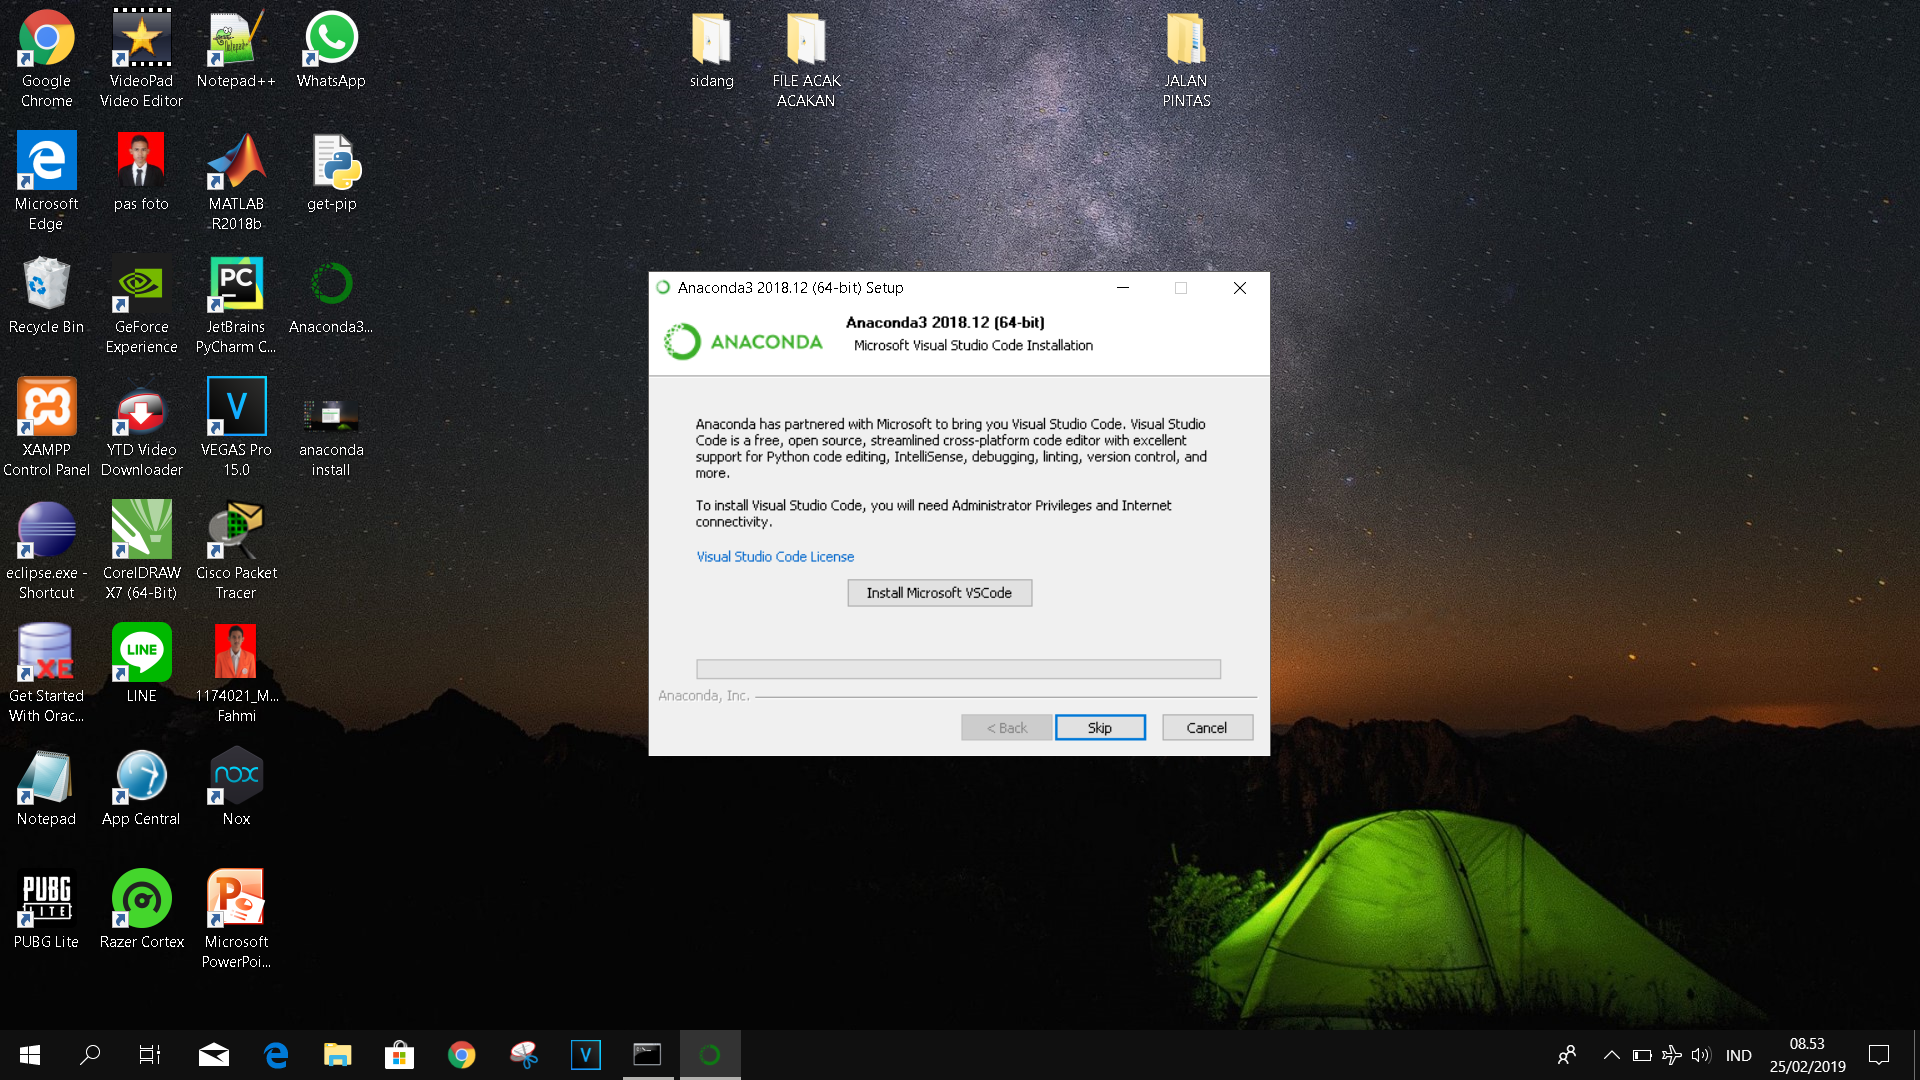
\includegraphics[width=3cm,height=3cm]{figures/2.png}
        \caption{gambar2}
        \label{next}
        \end{figure}

    \item Setelah itu setujui lisensi yang ada dengan mengklik I Agree
    \begin{figure}[!htbp]
        \centering
        \includegraphics[width=3cm,height=3cm]{figures/3.png}
        \caption{gambar3}
        \label{lisensi}
        \end{figure}

    \item Tunggu instalasi selesai, lalu klik skip
    \begin{figure}[!htbp]
        \centering
        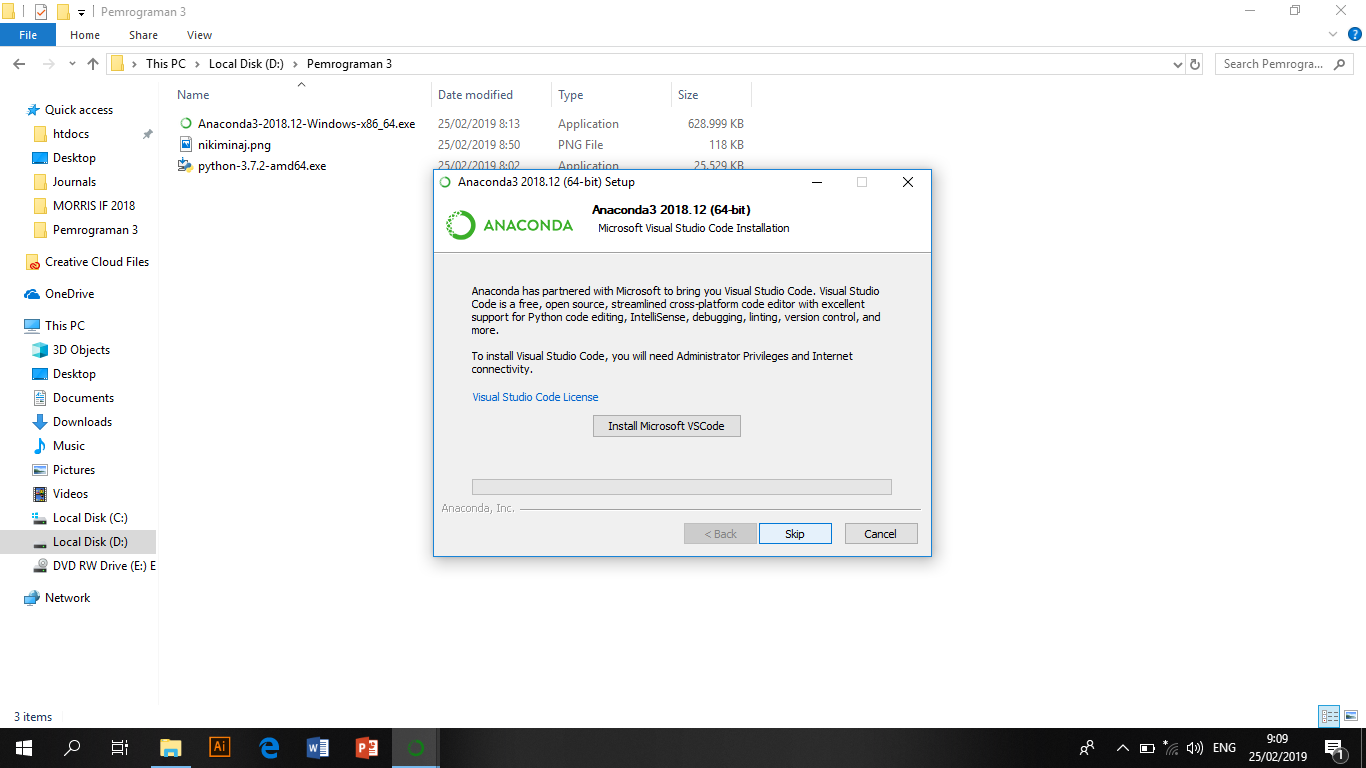
\includegraphics[width=3cm,height=3cm]{figures/4.png}
        \caption{gambar4}
        \label{skip}
        \end{figure}

    \item setelah itu klik finish, dan selesai yeay
    \begin{figure}[!htbp]
        \centering
        \includegraphics[width=3cm,height=3cm]{figures/5.png}
        \caption{gambar5}
        \label{selesai}
        \end{figure}
\end{enumerate}

\subsection{Menggunakan Spyder}
berikut adalah contoh dalam menggunakan spyder
\begin{figure}[!htbp]
    \centering
    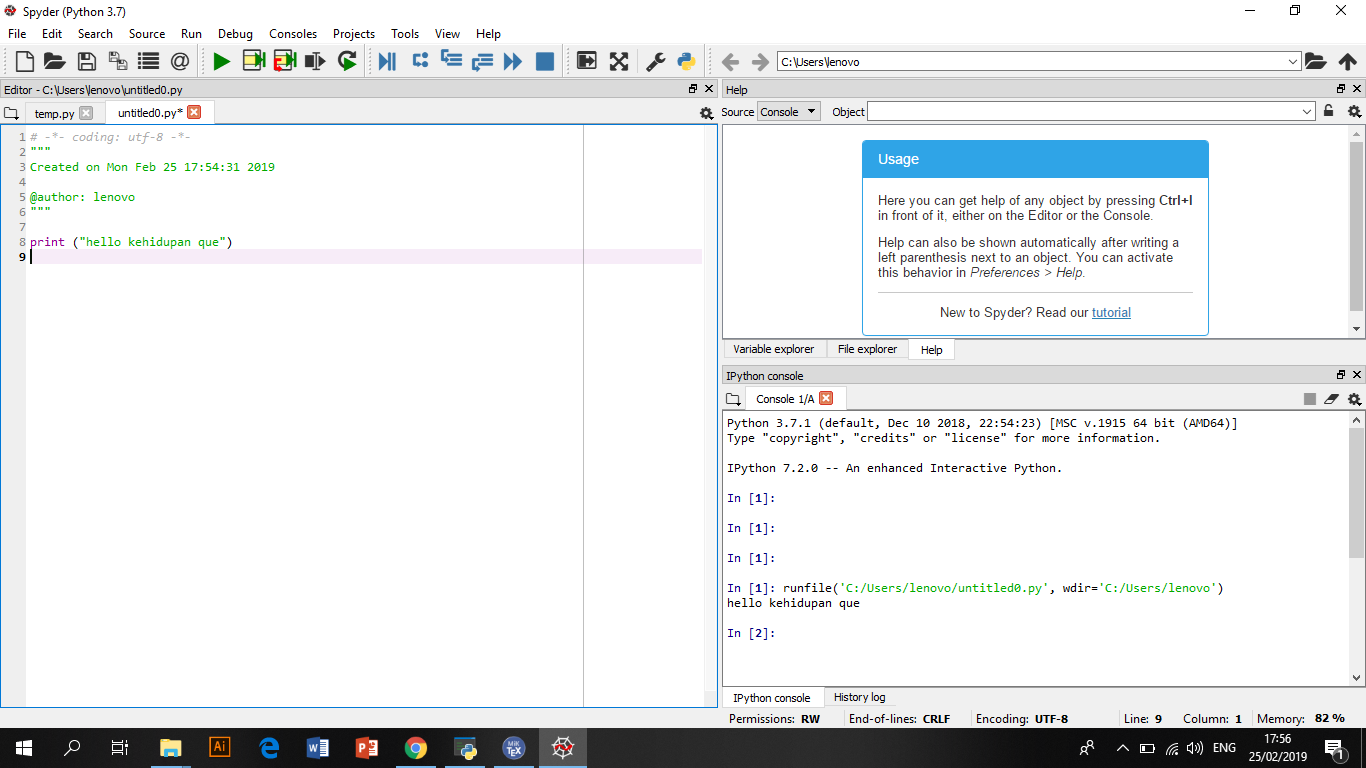
\includegraphics[width=3cm,height=3cm]{figures/6.png}
    \caption{gambar6}
    \label{spyder}
    \end{figure}
%%%%%%%%%%%%%%%%%%%%%%%%%%%%%%%%%%%%%%%%%%%%%%%%%%%%%%%	
\section{Dwi Septiani Tsaniyah}
\subsection{Sejarah Python}

Python dikembangkan oleh Guido van Rossum sebagai bahasa pemrograman ABC pada tahun 1990 di Stichting Mathematisch Centrum (CWI) di Amsterdam. Versi terbaru yang dirilis oleh CWI adalah 1.2.

Pada 1995, Guido pindah ke CNRI di Virginia, AS, dan terus mengembangkan Python. Versi terakhir yang dirilis 1.6. Pada tahun 2000, insinyur Guido dan Python menjadi perusahaan komersial untuk BeOpen.com dan menciptakan BeOpen PythonLabs. Python 2.0 dirilis oleh BeOpen. Setelah menghapus Python 2.0, beberapa anggota Guido dan PythonLabs pindah ke DigitalCreations.

Saat ini, pengembangan Python sedang dilanjutkan oleh sekelompok programmer yang dikoordinir oleh Guido dan Yayasan Perangkat Lunak Python. Python Software Foundation, versi 2.1, memiliki hak cipta Python, dan Python adalah organisasi nirlaba yang memblokir kepemilikan perusahaan komersial. Saat ini, distribusi Python telah mencapai versi 2.7.14 dan versi 3.6.3

Program televisi Guido Monty Python Flying Circus telah dinamai nama Python oleh Guido sebagai bahasa ciptaannya. Oleh karena itu, sering kali ungkapan khas suatu acara sering muncul dalam korespondensi antara pengguna Python.

\subsection{Instalasi Anaconda}
\begin{enumerate}
    \item Pastikan Bahwa Python telah terinstal dilaptop anda.
    \item Jika anda belum punya anaconda
    \item Kemudian buka installer yang telah di download barusan
    \item Klik next
    

    \item Kemudian Klik I Agree
    

    \item Kemudian pilih akan di instal untuk siapa, kemudian pilih next
    

    \item Kemudian tentukan dicretory nya
    

    \item Kemudian Centang yang register Anaconda as default Python, Kemudian Pilih Next
    

    \item Tunggu Proses Instalasi hingga selesai
    

    \item Instalasi telah selesai
	\end{enumerate}
    
\subsection{Penggunaan Spyder}
kodingan sederhana Hello Word 

%%%%%%%%%%%%%%%%%%%%%%%%%%%%%%%%%%%%%%%%%%%%%%%%%%%%%%%%%%%%%%%%%%

\section{Kadek Diva Krishna Murti}

\subsection{Sejarah Python}
Python merupakan salah satu bahasa pemrograman tingkat tinggi yang menggunakan metode pemrosesan \textit{interpreted}, dimana kode program akan diproses baris per baris secara langsung dari kode program.

Bahasa pemrograman Python dirilis pertama kali oleh Guido van Rossum di Scitchting Mathematisch Centrum (CWI) Belanda pada tahun 1991. Bahasa python terinspirasi dari bahasa pemrograman ABC. Nama python tidak berasal dari nama ular yang kita kenal. Guido merupakan penggemar grup komedi Inggris bernama Monty Python. Kemudian, ia menamakan Bahasa pemrograman ciptaannya dengan nama Python.

Pada tahun 1994, Python 1.0 dirilis, yang diikuti dengan Python 2.0 pada tahun 2000. Python 3.0 keluar pada tahun 2008. Sampai saat ini Python masih dikembangkan oleh \textit{Python Software Foundation}. Bahasa Python mendukung hampir semua sistem operasi, bahkan untuk sistem operasi Linux, hampir semua distronya sudah menyertakan Python di dalamnya \cite{roihan2017monitoring}.


\subsection{Instalasi Anaconda}
Berikut ini merupakan langkah-langkah cara instalasi Anaconda di windows:
\begin{enumerate}
	\item Pastikan kalian telah menginstall Python sebelumnya.
	\item Klik dua kali pada installer Anaconda. Installer anaconda bisa anda dapatkan di https://www.anaconda.com/distribution/
	\item Setelah itu akan muncul window installernya. Kemudian klik ''Next'' untuk memulai instalasi.
	\begin{figure}[H]
		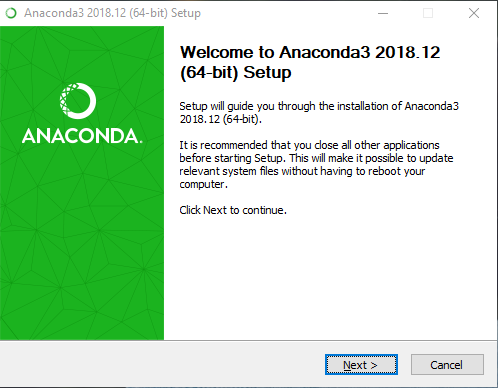
\includegraphics[width=10cm]{figures/diva/1chp1diva.png}
		\centering
	\end{figure}

	\item Baca Lisensi Agreement Anacondanya. Lalu klik ''I Agree'' jika kalian menerimanya dan untuk melajutkannya instalasinya.
	\begin{figure}[H]
		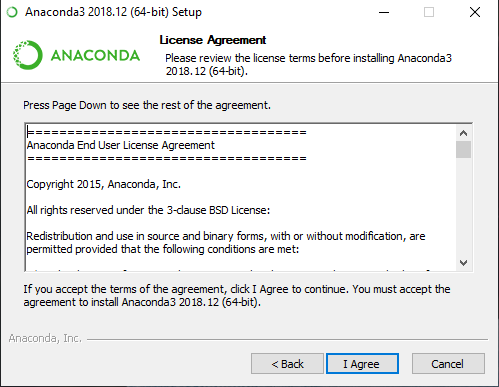
\includegraphics[width=10cm]{figures/diva/2chp1diva.png}
		\centering
	\end{figure}

	\item Selanjutnya diberi pilihan untuk menginstallnya, apakah hanya untuk kalian atau untuk semua pengguna. Disini saya memilih ''All Users'', lalu klik ''Next''.
	\begin{figure}[H]
		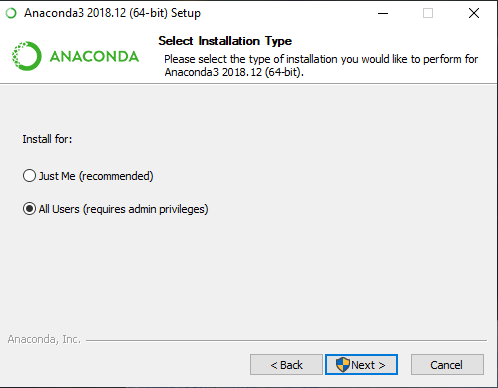
\includegraphics[width=10cm]{figures/diva/3chp1diva.png}
		\centering
	\end{figure}

	\item Kemudian pilih tujuan instalasinya. Disini saya biarkan default folder instalasinya. Setelah itu, klik ''Next''.
	\begin{figure}[H]
		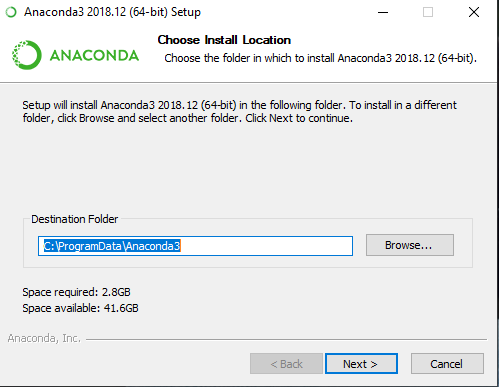
\includegraphics[width=10cm]{figures/diva/4chp1diva.png}
		\centering
	\end{figure}

	\item Setelah itu, kalian diberi beberapa opsi tambahan. Opsi pertama yaitu, ''Add Anaconda to my PATH environment variable''. Opsi ini akan menambahkan Anaconda ke PATH sistem environment variable. Opsi kedua yaitu, ''Register Anaconda as my default Python 3.7''. Opsi ini akan mendaftarkan Anaconda sebagai system Python 3.7. Saya centang kedua opsi tersebut, lalu klik ''Install''.
	\begin{figure}[H]
		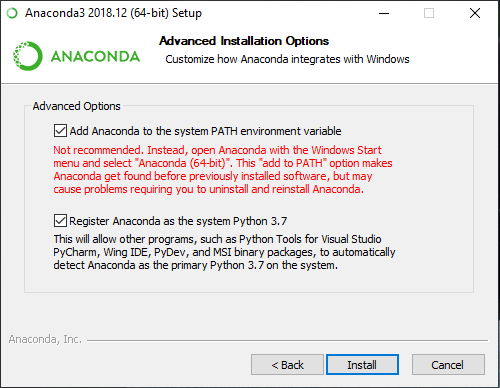
\includegraphics[width=10cm]{figures/diva/5chp1diva.png}
		\centering
	\end{figure}

	\item Tunggu hingga proses instalasi selesai.
	\begin{figure}[H]
		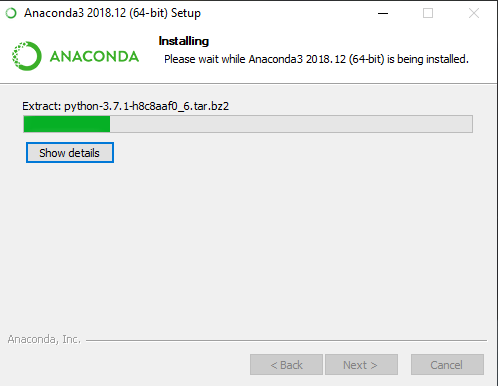
\includegraphics[width=10cm]{figures/diva/6chp1diva.png}
		\centering
	\end{figure}

	\item Kemudian klik ''Next'' untuk melanjutkan.
	\begin{figure}[H]
		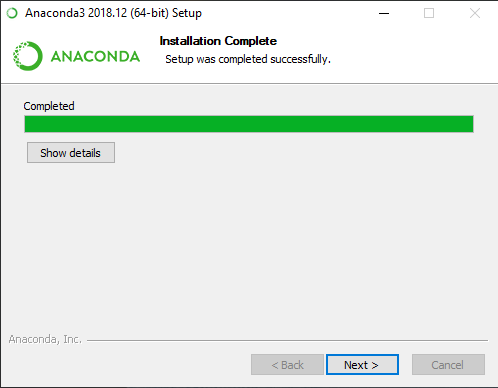
\includegraphics[width=10cm]{figures/diva/7chp1diva.png}
		\centering
	\end{figure}

	\item Selanjutnya kalian diberi pilihan untuk menginstall Microsoft VSCode. Saya klik ''Skip'' untuk melanjutkan.
	\begin{figure}[H]
		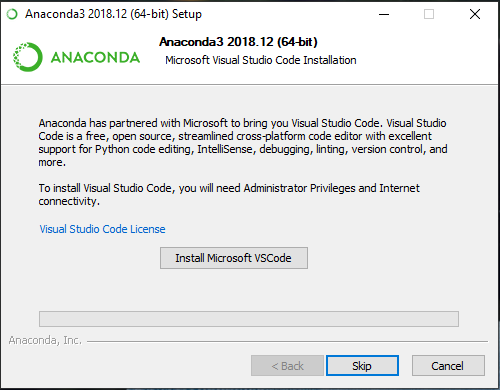
\includegraphics[width=10cm]{figures/diva/8chp1diva.png}
		\centering
	\end{figure}

	\item Kemudian klik ''Finish'' untuk selesai.
	\begin{figure}[H]
		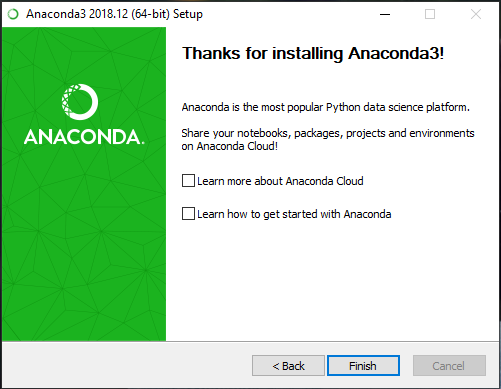
\includegraphics[width=10cm]{figures/diva/9chp1diva.png}
		\centering
	\end{figure}

	\item Untuk mengecek apakah Anaconda telah terinstall yaitu dengan cara membuka Command Prompt. Lalu ketikan ''conda -V'' dan tekan enter, kode itu akan mengecek versi Anaconda yang terinstall.
	\begin{figure}[H]
		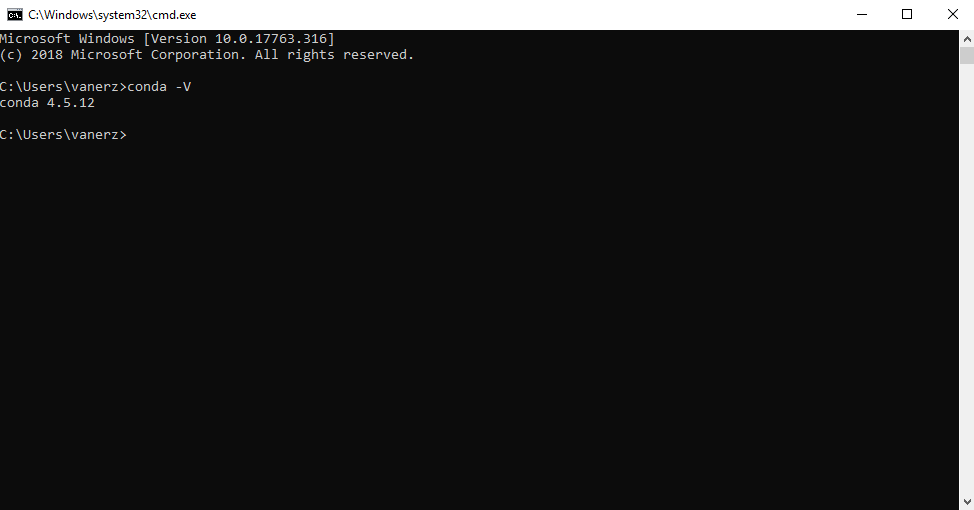
\includegraphics[width=10cm]{figures/diva/10chp1diva.png}
		\centering
	\end{figure}

\end{enumerate}

\subsection{Penggunaan Spyder}

Terdapat 2 cara menjalankan Spyder. Yang pertama dengan Anaconda Prompt dan yang kedua dengan Anaconda Navigation. Berikut ini merupakan langkah-langkah cara menjalankan Spyder di windows:

\begin{itemize}
	\item Anaconda Prompt

	\begin{enumerate}
		
		\item Pertama klik start, lalu cari ''Anaconda Prompt''.
		\begin{figure}[H]
			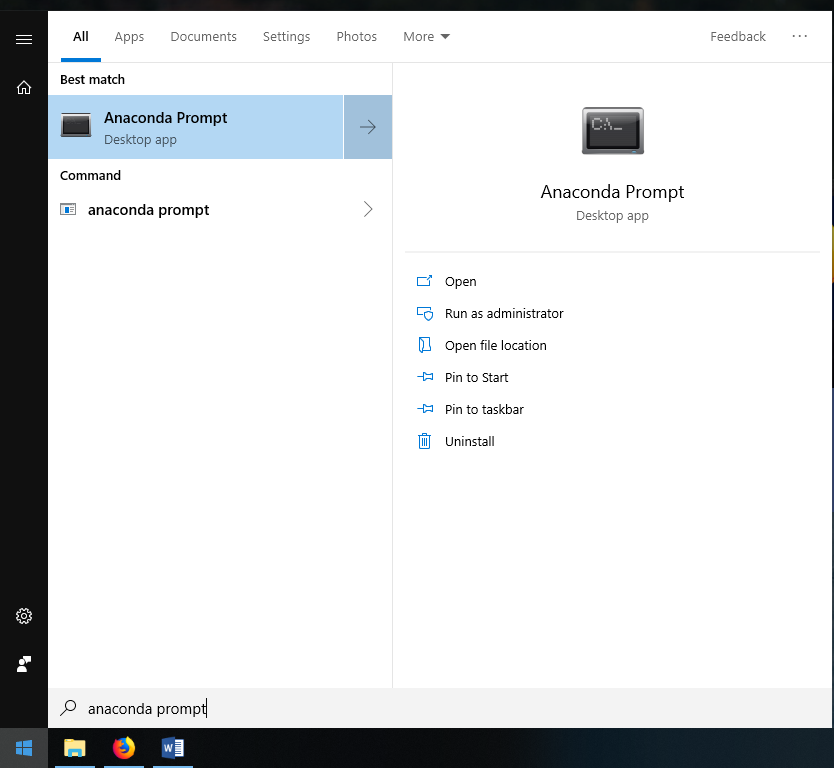
\includegraphics[width=10cm]{figures/diva/11chp1diva.png}
			\centering
		\end{figure}		
		\item Selanjutnya akan muncul sebuah prompt. Kemudian ketikan ''start spyder'' dan tekan enter.
		\begin{figure}[H]
			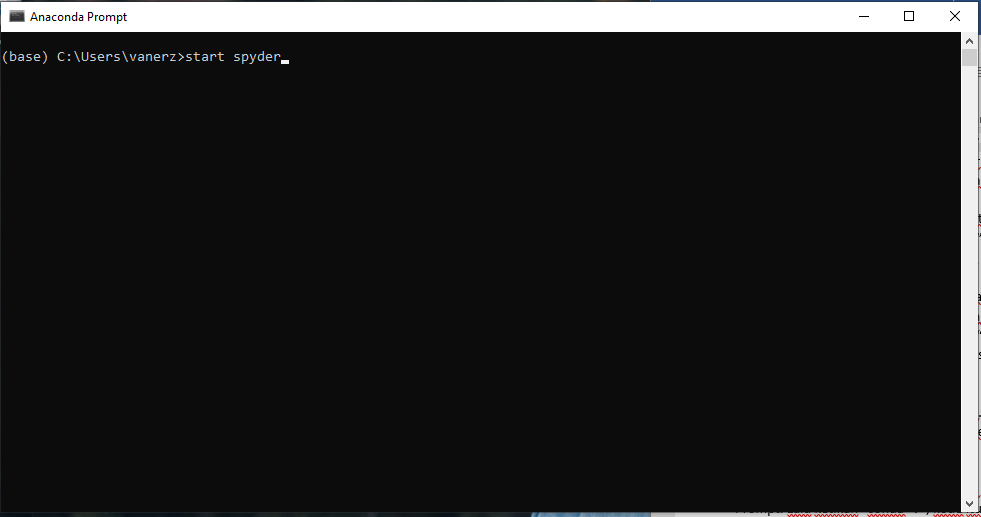
\includegraphics[width=10cm]{figures/diva/12chp1diva.png}
			\centering
		\end{figure}
		\item Lalu tunggu sampai selesai.
		\begin{figure}[H]
			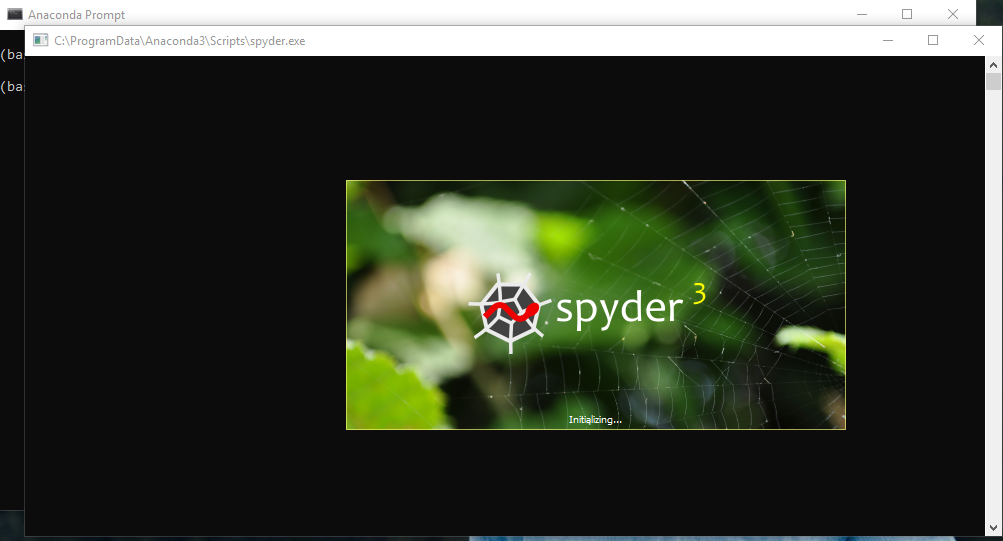
\includegraphics[width=10cm]{figures/diva/13chp1diva.png}
			\centering
		\end{figure}

	\end{enumerate}
	\item Anaconda Navigation

	\begin{enumerate}
		\item Pertama klik start, lalu cari ''Anaconda Navigation''.
		\begin{figure}[H]
			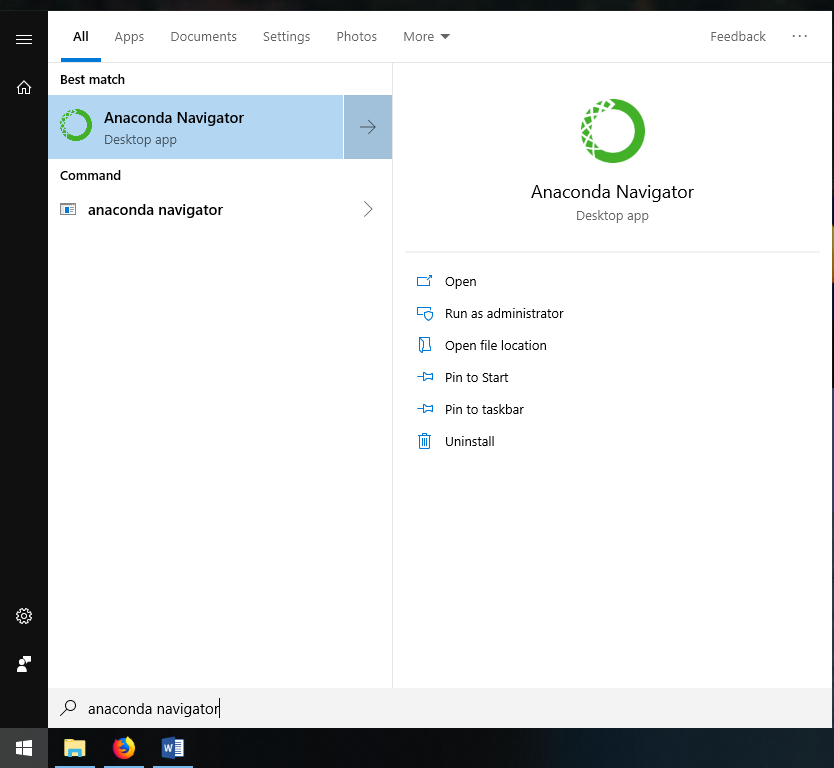
\includegraphics[width=10cm]{figures/diva/14chp1diva.png}
			\centering
		\end{figure}
		\item Selanjutnya akan muncul sebuah window. Kemudian klik ''Launch'' pada menu Spyder.
		\begin{figure}[H]
			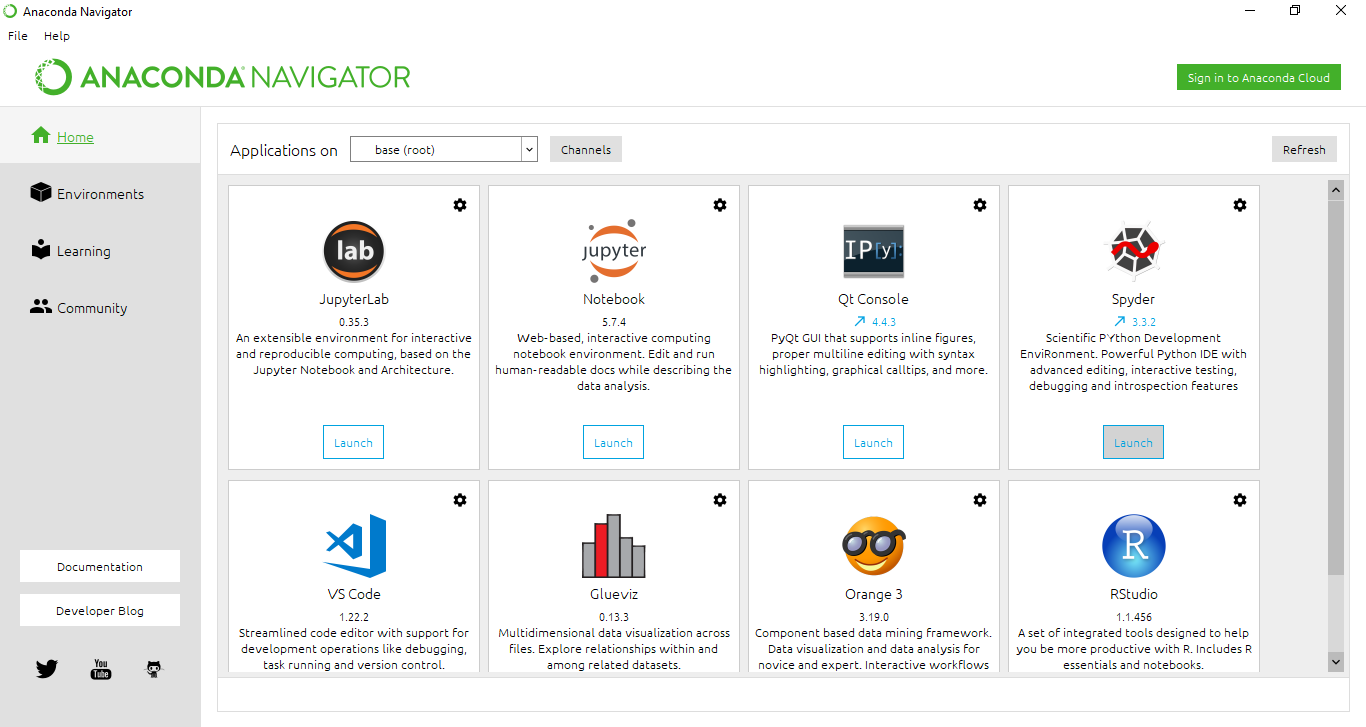
\includegraphics[width=10cm]{figures/diva/15chp1diva.png}
			\centering
		\end{figure}
		\item Lalu tunggu sampai selesai.
		\begin{figure}[H]
			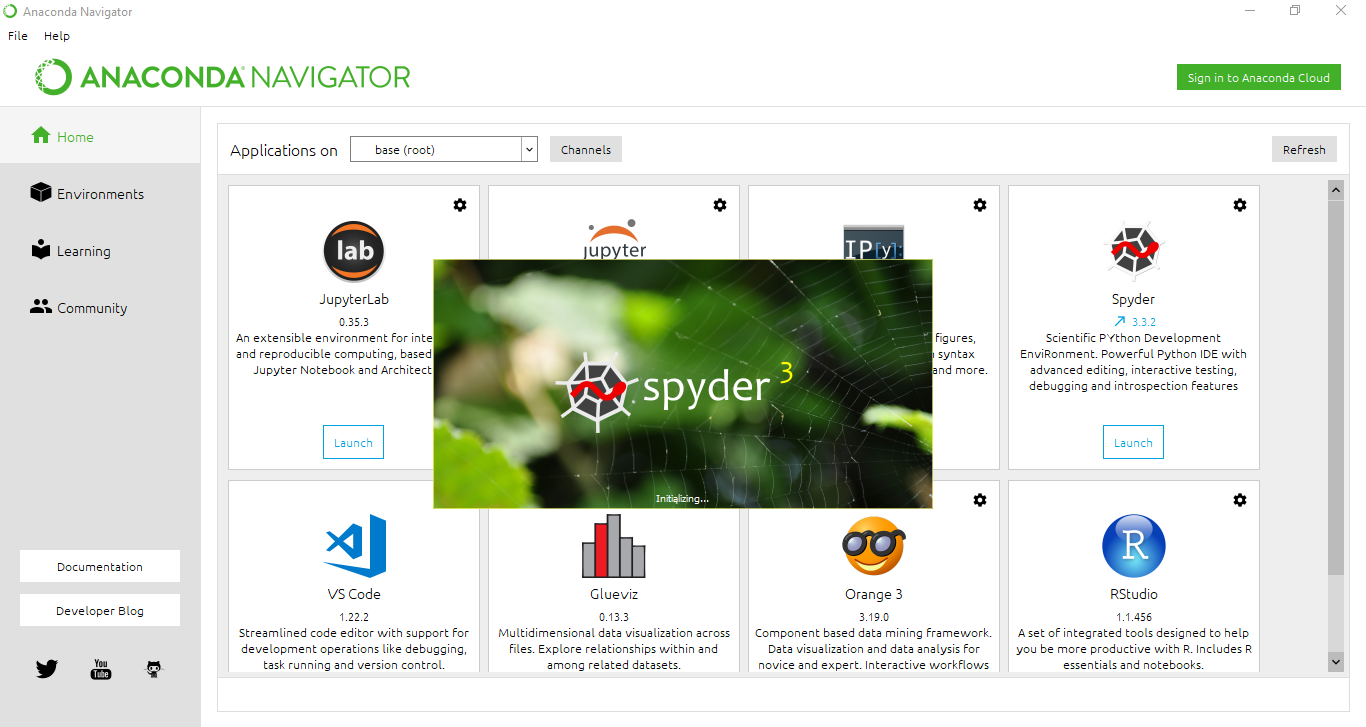
\includegraphics[width=10cm]{figures/diva/16chp1diva.png}
			\centering
		\end{figure}

	\end{enumerate}
\end{itemize}

Apabila muncul window in ketika pertama kali menjalankan Spyder, pilih “Allow Access”.
\begin{figure}[H]
	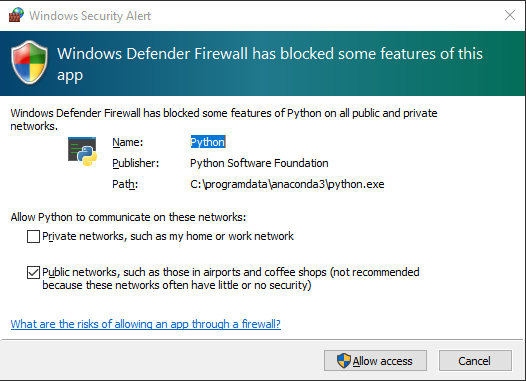
\includegraphics[width=10cm]{figures/diva/17chp1diva.png}
	\centering
\end{figure}
		
Berikut ini merupakan gambar dari Spyder
\begin{figure}[H]
	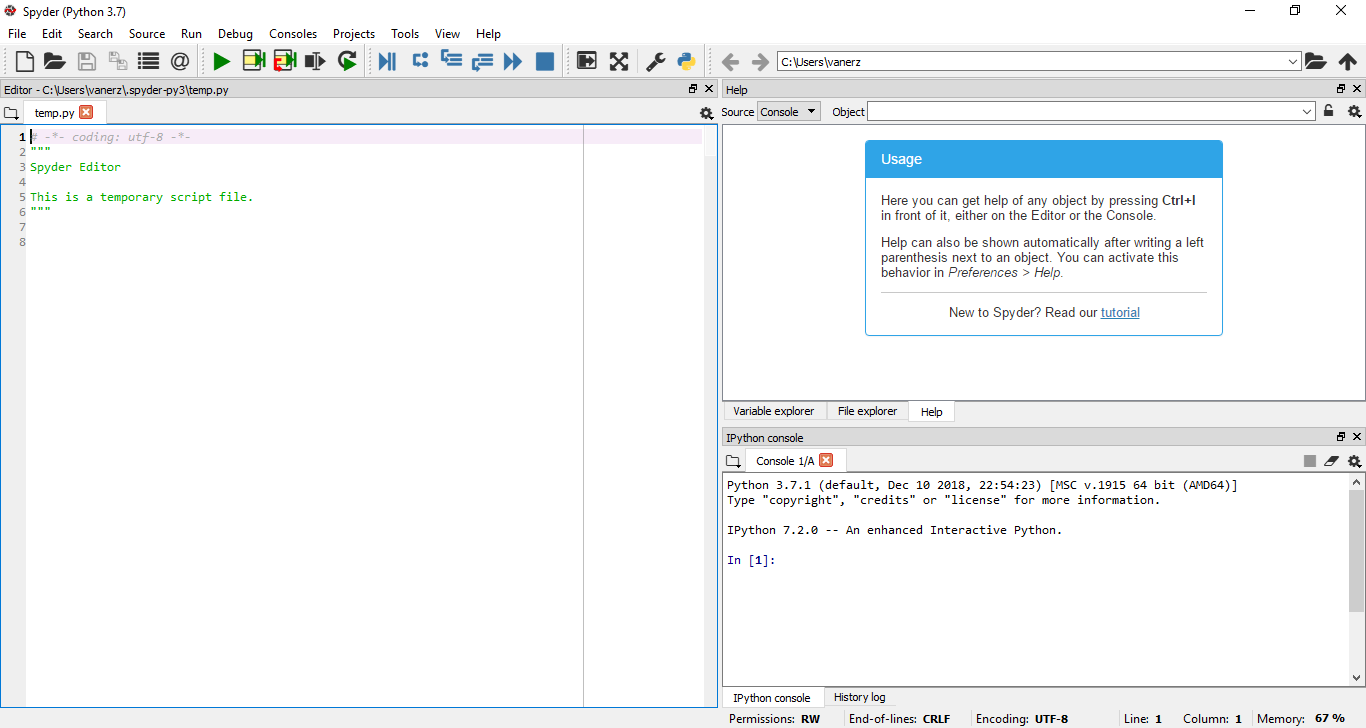
\includegraphics[width=10cm]{figures/diva/18chp1diva.png}
	\centering
\end{figure}

Berikut cara menggunakan Spyder:
\begin{enumerate}
	\item Silahkan ketikan script Python anda di sini.
	\begin{figure}[H]
		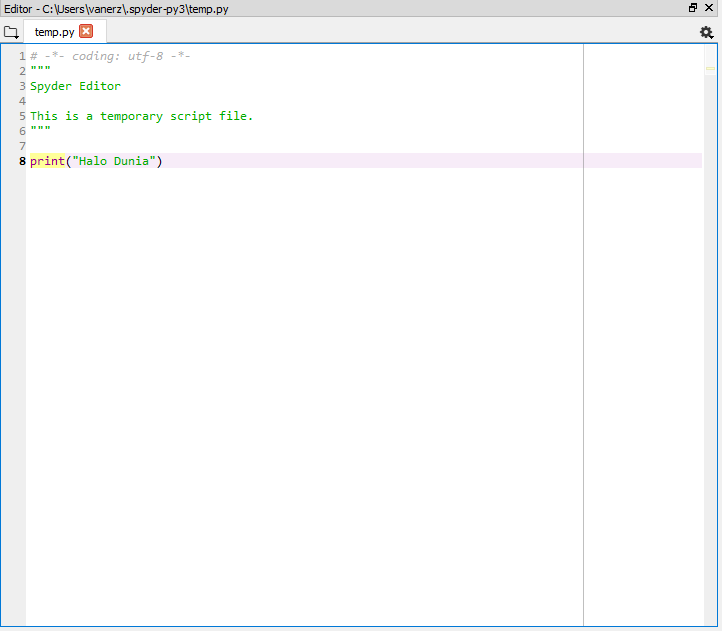
\includegraphics[width=10cm]{figures/diva/20chp1diva.png}
		\centering
	\end{figure}
	\item Setelah mengetik script Python, kemudian klik tombol play atau tekan tombol F5 untuk mengeksekusi script Python yang telah diketik tadi.
	\begin{figure}[H]
		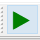
\includegraphics[width=2cm]{figures/diva/22chp1diva.png}
		\centering
	\end{figure}
	\item Hasil dari eksekusi akan muncul disini.
	\begin{figure}[H]
		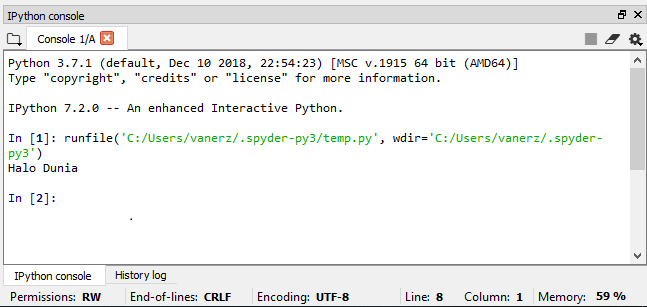
\includegraphics[width=10cm]{figures/diva/21chp1diva.png}
		\centering
	\end{figure}
		\item Berikut tampilan penuhnya.
	\begin{figure}[H]
		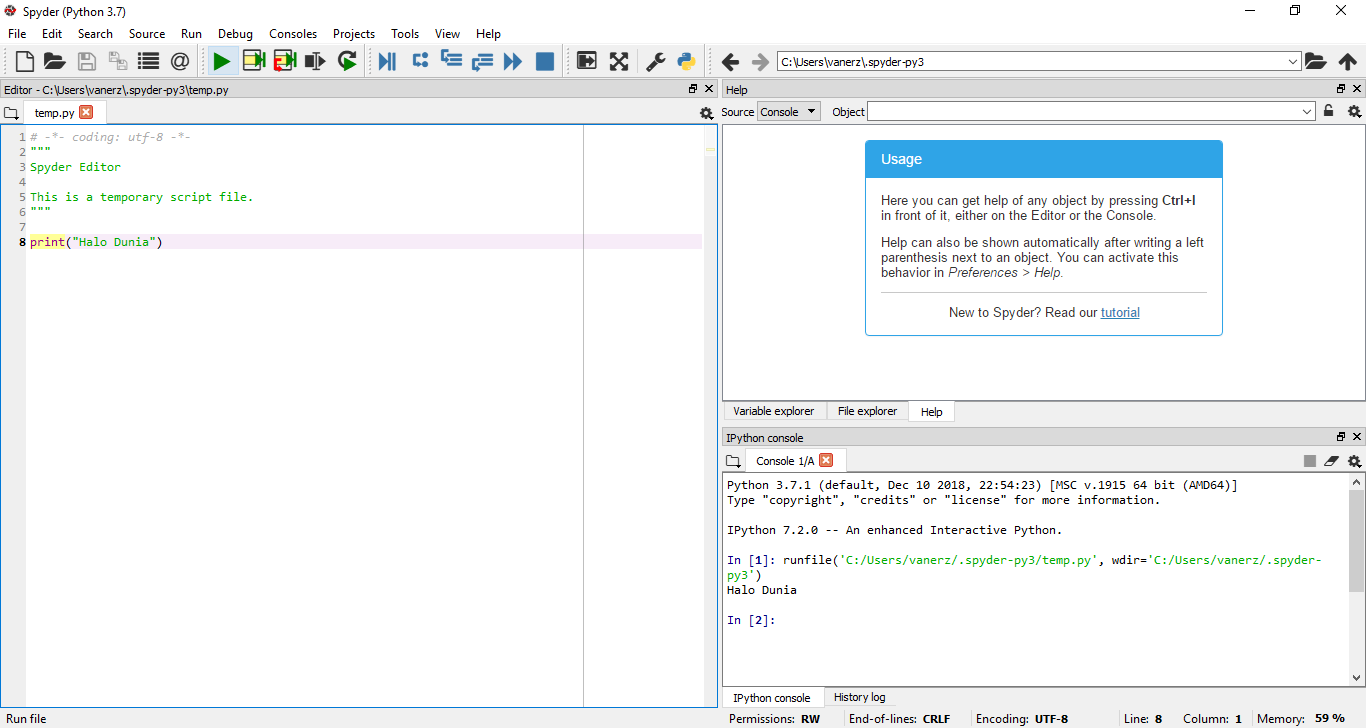
\includegraphics[width=10cm]{figures/diva/19chp1diva.png}
		\centering
	\end{figure}
\end{enumerate}

%%%%%%%%%%%%%%%%%%%%%%%%%%%%%%%%%%%%%%%%

\section{Harun Ar-Rasyid}
\subsection{Sejarah}
Python diciptakan oleh Guido van Rossum pertama kali di Scitchting Mathematisch Centrum (CWI) di Belanda pada awal tahun 1990-an. Bahasa python terinspirasi dari bahasa pemrograman ABC. Sampai sekarang, Guido masih menjadi penulis utama untuk python, meskipun bersifat open source sehingga ribuan orang juga berkontribusi dalam mengembangkannya.

Pada 1995, Guido pindah ke CNRI di Virginia Amerika sambil terus mengembangkan Python. Versi terakhir yang dirilis adalah 1.6. Pada tahun 2000, pengembang inti Guido dan Python pindah ke BeOpen.com yang merupakan perusahaan komersial dan membentuk BeOpen PythonLabs. Python 2.0 dirilis oleh BeOpen. Setelah menghapus Python 2.0, Guido dan beberapa anggota tim PythonLabs pindah ke DigitalCreations.

Saat ini pengembangan Python terus dilakukan oleh sekelompok programmer yang dikoordinir oleh Guido dan Python Software Foundation. Python Software Foundation adalah organisasi nirlaba yang dibentuk sebagai pemegang hak cipta intelektual Python sejak versi 2.1 dan dengan demikian mencegah Python dimiliki oleh perusahaan komersial. Saat ini distribusi Python telah mencapai versi 2.7.14 dan versi 3.6.3

Nama Python dipilih oleh Guido sebagai nama bahasa ciptaannya karena kecintaan Guido pada acara televisi Flying Circus Monty Python. Oleh karena itu sering ekspresi khas acara sering muncul dalam korespondensi antara pengguna Python.
\subsection{Instalasi Anaconda}
\begin{enumerate}
    \item Pastikan Bahwa Python telah terinstal dilaptop anda.
    \item Kemudian Download Anaconda pada websitenya langsung.
    \item Kemudian buka installer yang telah di download barusan
    \item Klik next
    \begin{figure}[!Htbp]
        \centering
        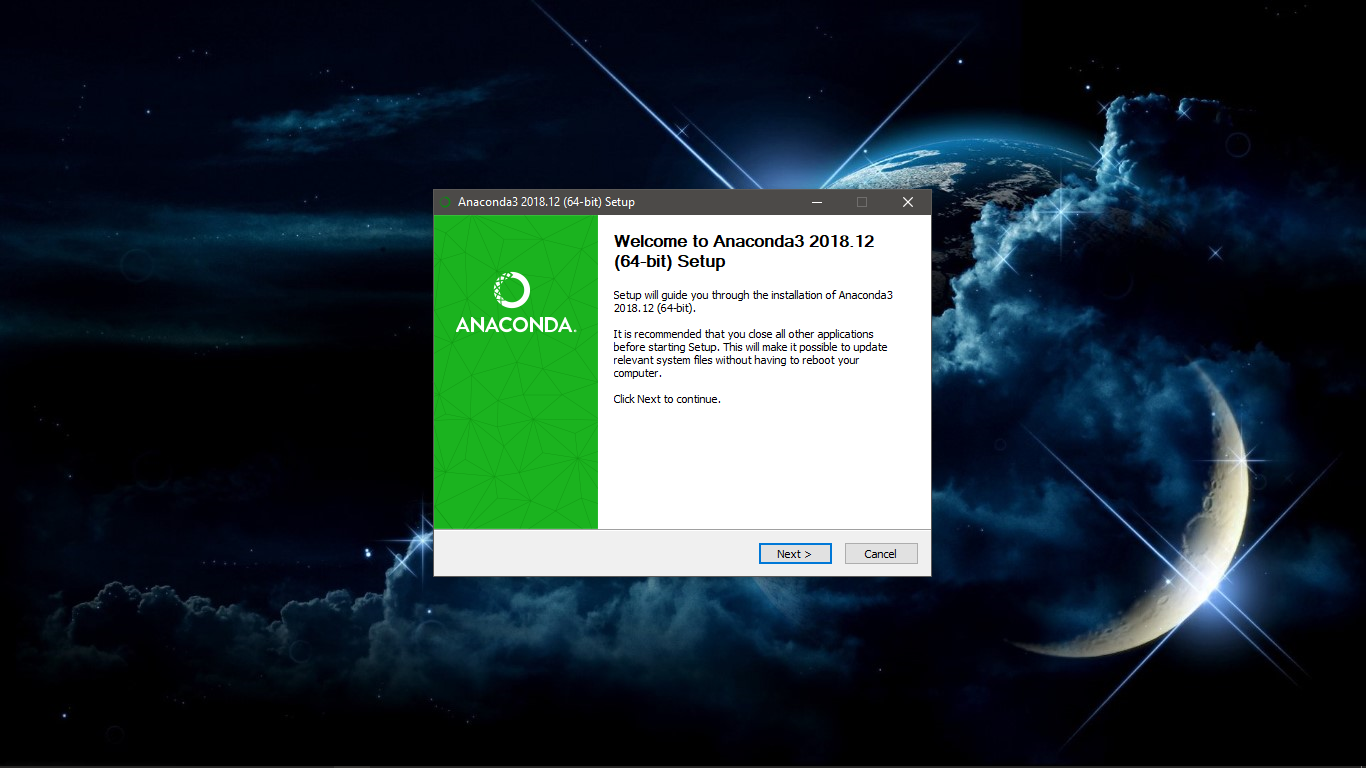
\includegraphics[width=3cm,height=3cm]{figures/Screenshot(80).png}
        \caption{Tampilan Awal}
        \label{awal}
        \end{figure}

    \item Kemudian Klik I Agree
    \begin{figure}[!Htbp]
        \centering
        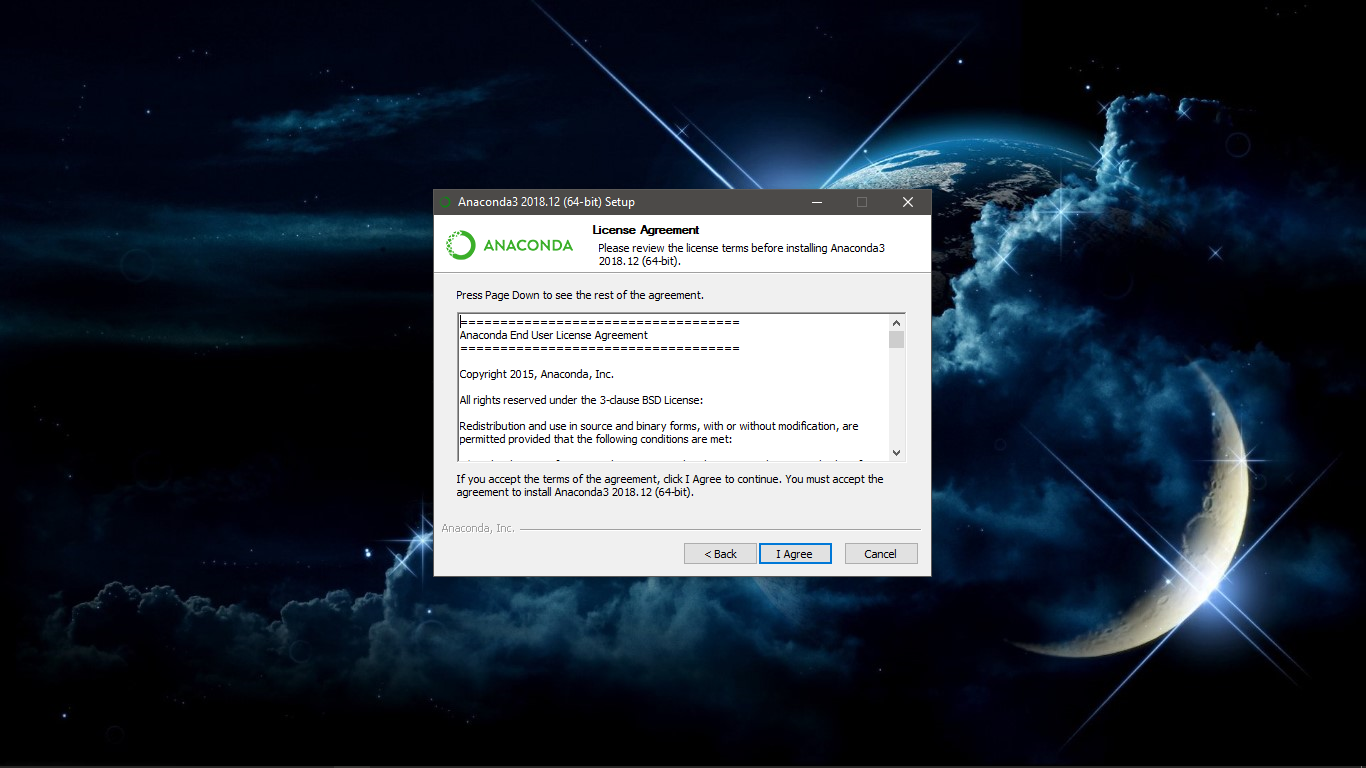
\includegraphics[width=3cm,height=3cm]{figures/Screenshot(81).png}
        \caption{License Agreement}
        \label{License}
        \end{figure}

    \item Kemudian pilih akan di instal untuk siapa, kemudian pilih next
    \begin{figure}[!Htbp]
        \centering
        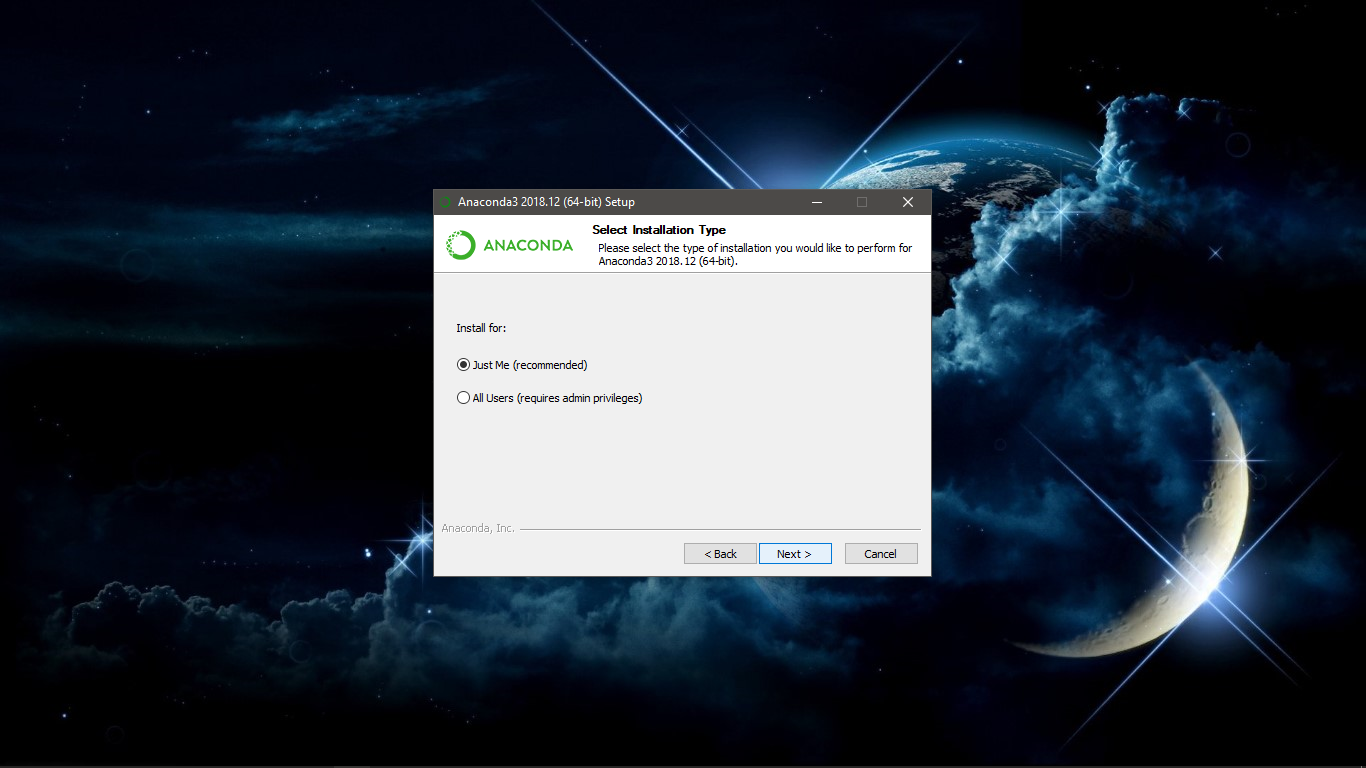
\includegraphics[width=3cm,height=3cm]{figures/Screenshot(82).png}
        \caption{Pemilihan User}
        \label{User}
        \end{figure}

    \item Kemudian tentukan dicretory nya
    \begin{figure}[!Htbp]
        \centering
        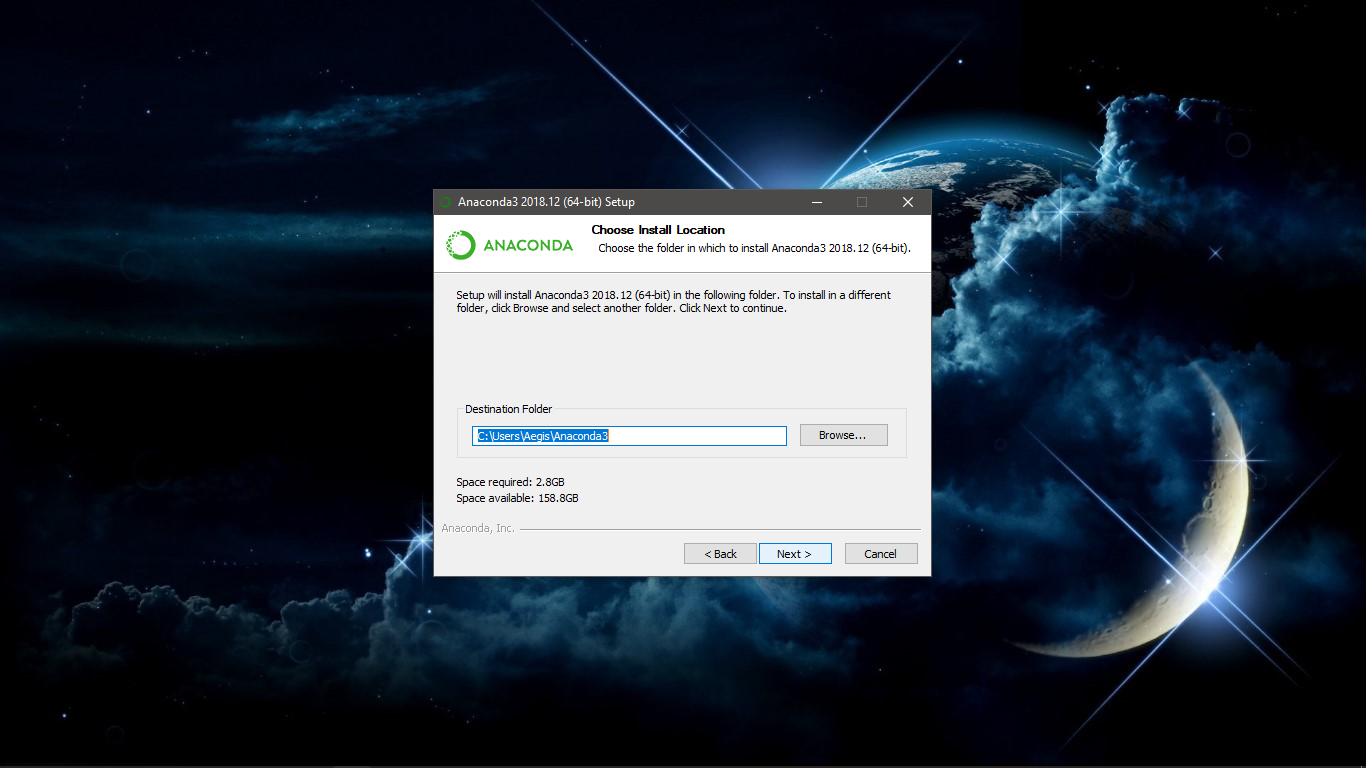
\includegraphics[width=3cm,height=3cm]{figures/Screenshot(83).png}
        \caption{Pemilihan Direktori Penyimpanan}
        \label{Directory}
        \end{figure}

    \item Kemudian Centang yang register Anaconda as default Python, Kemudian Pilih Next
    \begin{figure}[!Htbp]
        \centering
        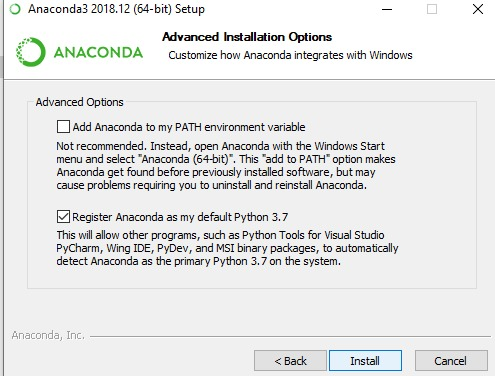
\includegraphics[width=3cm,height=3cm]{figures/Screenshot(84).jpeg}
        \caption{Pemilihan Opsi}
        \label{opsi}
        \end{figure}

    \item Tunggu Proses Instalasi hingga selesai
    \begin{figure}[!Htbp]
        \centering
        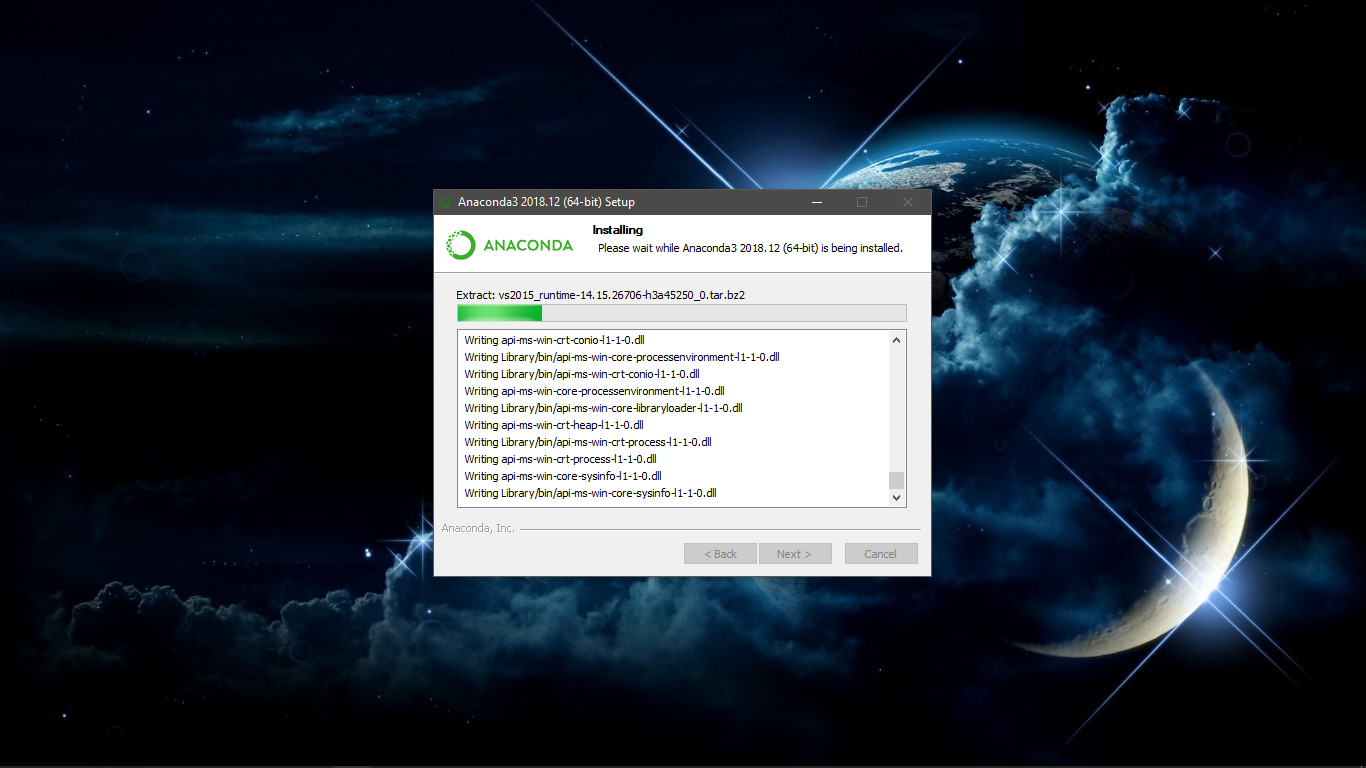
\includegraphics[width=3cm,height=3cm]{figures/Screenshot(85).png}
        \caption{Proses Instal}
        \label{Proses}
        \end{figure}

    \item Klik next
    \begin{figure}[!Htbp]
        \centering
        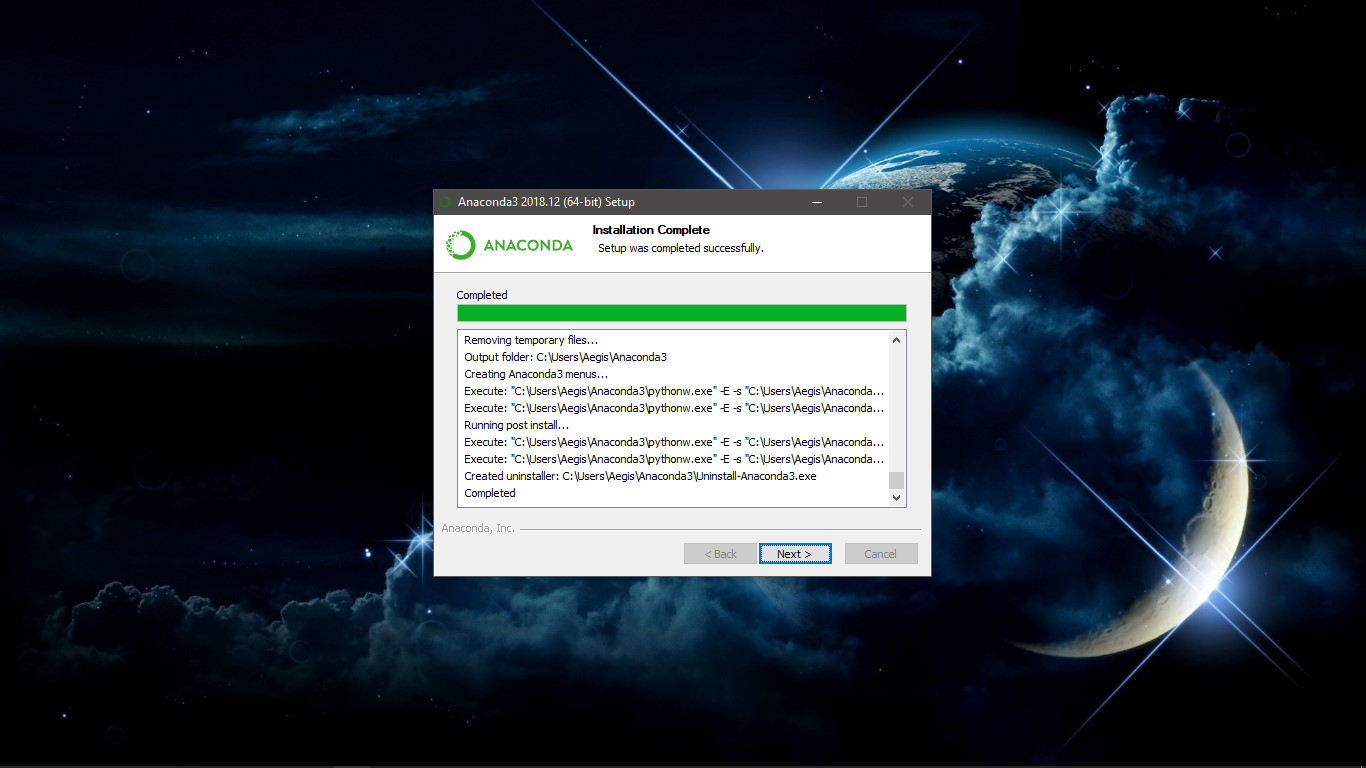
\includegraphics[width=3cm,height=3cm]{figures/Screenshot(86).png}
        \caption{Proses Instal Selesai}
        \label{Proses}
        \end{figure}

    \item kemudian jika kalian belum instal MS VSC di sarankan menginstalnya dlu, jika sudah klik skip
    \begin{figure}[!Htbp]
        \centering
        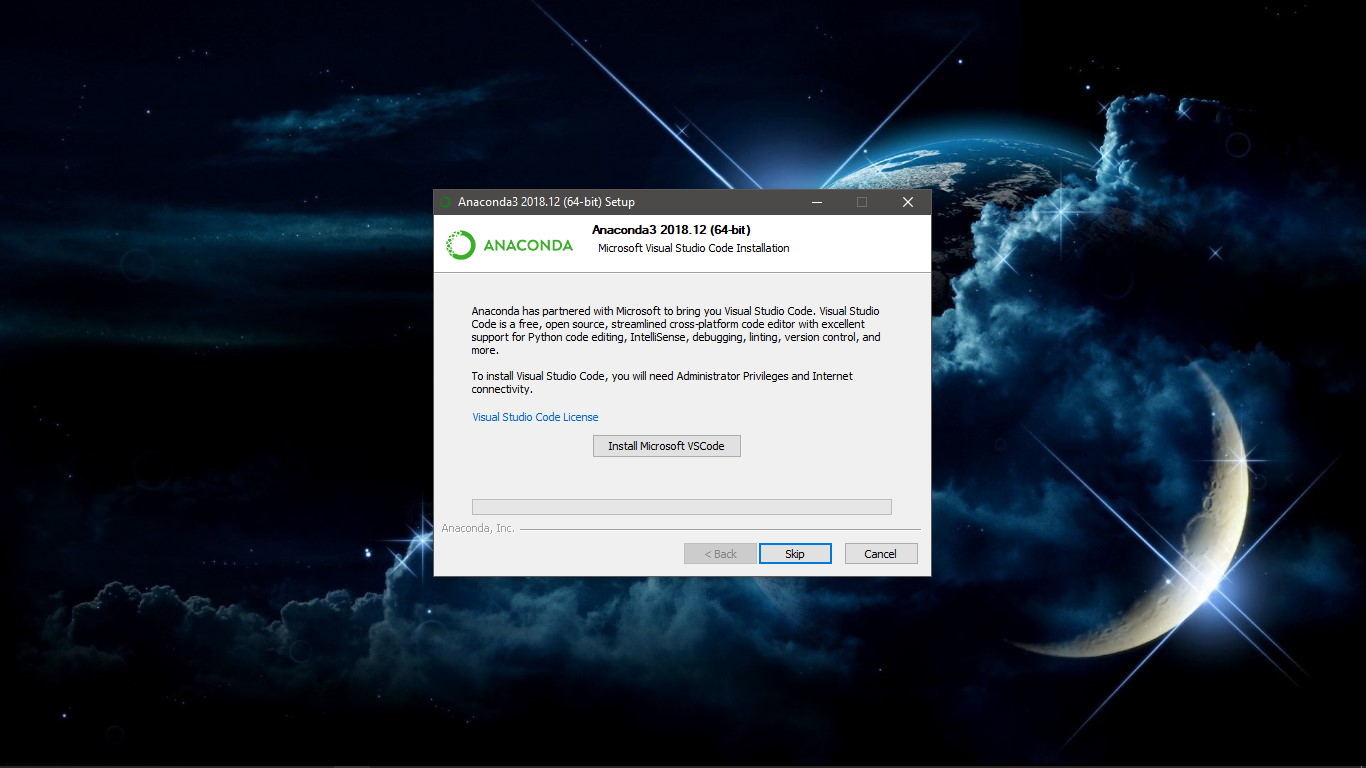
\includegraphics[width=3cm,height=3cm]{figures/Screenshot(87).png}
        \caption{Penawaran Instal MS VSC}
        \label{offering}
        \end{figure}

    \item Instalasi anaconda telah selesai
    \begin{figure}[!Htbp]
        \centering
        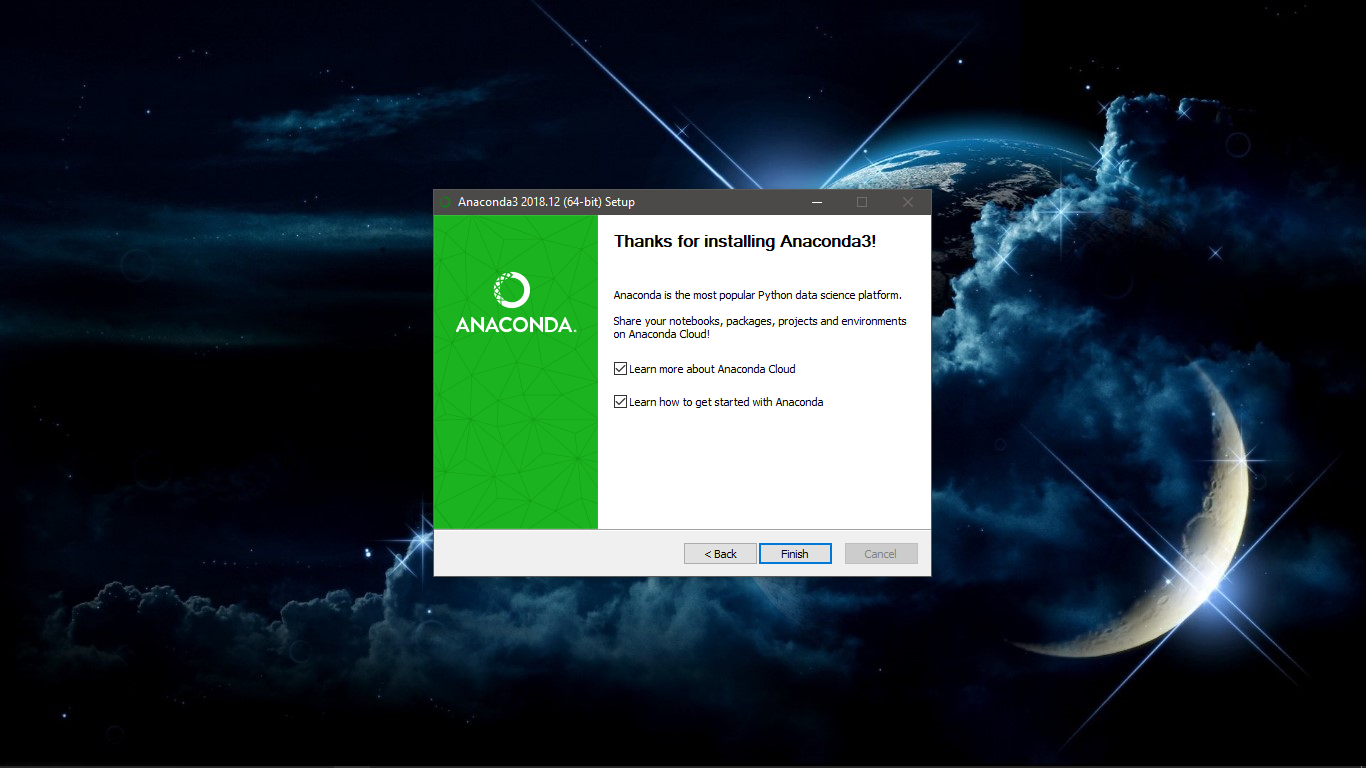
\includegraphics[width=3cm,height=3cm]{figures/Screenshot(88).png}
        \caption{Instalasi Selesai}
        \label{akhir}
        \end{figure}
\end{enumerate}
\subsection{Menggunakan Spyder}
Setelah selesai melakukan instalasi anaconda, maka ada beberapa tool yang digunakan seperti spyder

\begin{figure}[!Htbp]
    \centering
    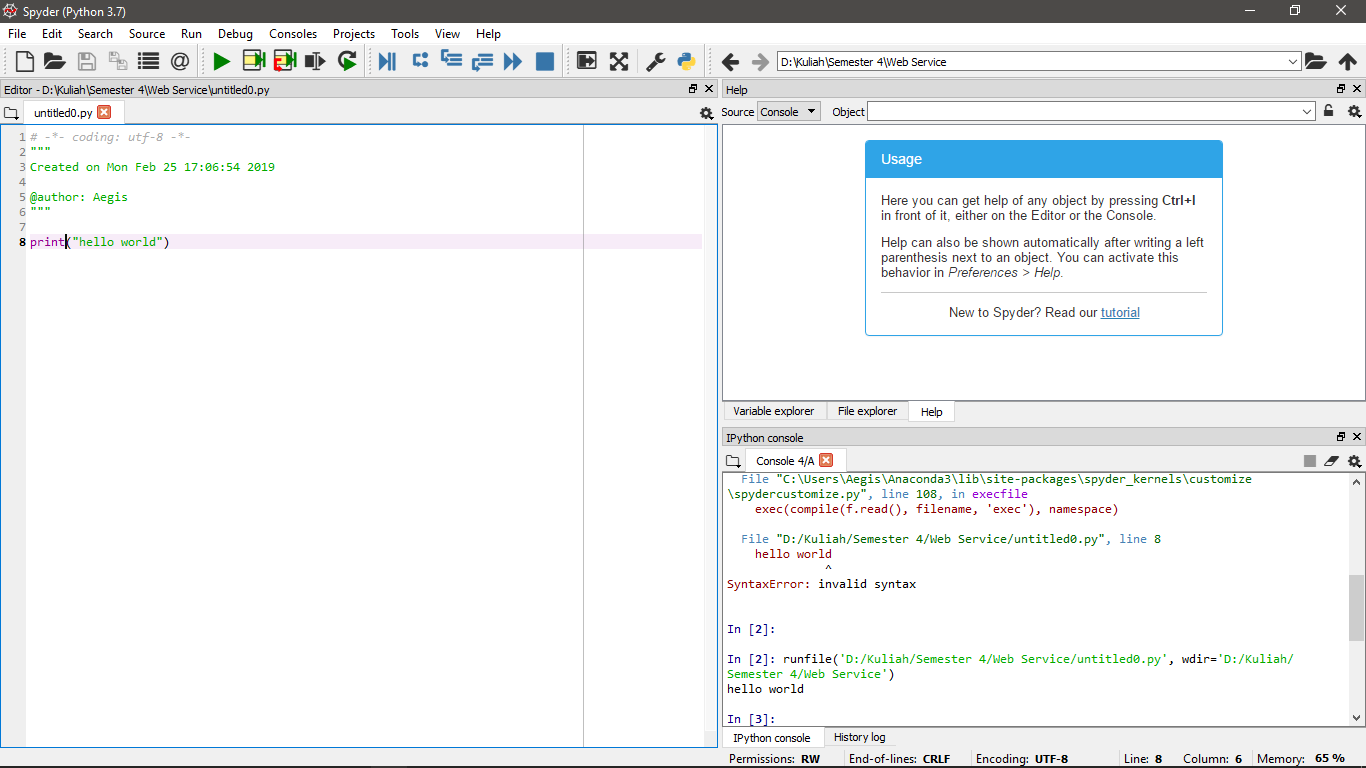
\includegraphics[width=3cm,height=3cm]{figures/Spyder.png}
    \caption{Ini adalah tampilan spyder}
    \label{spyder}
    \end{figure}

Gambar diatas menjelaskan tentang tampilan spider dan mengexsekusi program halo world.

%%%%%%%%%%%%%%%%%%%%%%%%%%%%%%%%%%%%%%%%%%%%

\section{Felix Lase}
\subsection{sejarah}
Python diciptakan oleh Guido van Rossum untuk pertama kalinya di Scitchting Mathematisch Centrum (CWI) di Belanda pada awal 1990-an. Bahasa Python terinspirasi oleh bahasa pemrograman ABC. Sampai sekarang, Guido masih menjadi penulis utama untuk Python, meskipun open source terbuka untuk ribuan orang yang juga berkontribusi pada pengembangannya.
\par
Pada tahun 1995, Guido terus membuat python di Corporate for National Research Initiative (CNRI) di Virginia America, tempat ia merilis beberapa versi Python.
\par
Pada bulan Mei 2000, Guido dan tim Python pindah ke BeOpen.com dan membentuk tim BeOpen PythonLabs. Pada bulan Oktober tahun yang sama, tim Python pindah ke Digital Creation (sekarang Zope Company). Pada tahun 2001, Organisasi Python dibentuk, Yayasan Perangkat Lunak Python (PSF). PSF adalah organisasi nirlaba yang khusus dibuat untuk semua hal yang berkaitan dengan kekayaan intelektual Python. Perusahaan Zope adalah anggota sponsor PSF.
\par
Semua versi Python yang dirilis adalah open source. Dalam sejarahnya, hampir semua rilis python menggunakan lisensi yang kompatibel dengan GFL. Berikutnya adalah versi minor dari walikota dan python bersama dengan tanggal rilis.Instalasi anaconda
\subsection{Instalasi Anaconda}
\begin{enumerate}
    \item Terlebih dahulu kita harus mendownload python, sebelum anaconda diinstal
    \item Buka installer klik Next
     \begin{figure}[!htbp]
        \centering
        \includegraphics[width=3cm,height=3cm]{figures/felix/1.png}
        \caption{Tampilan Awal}
        \label{awal}
        \end{figure}
    \item Klik I Agree untuk membuka lisensi
     \begin{figure}[!htbp]
        \centering
        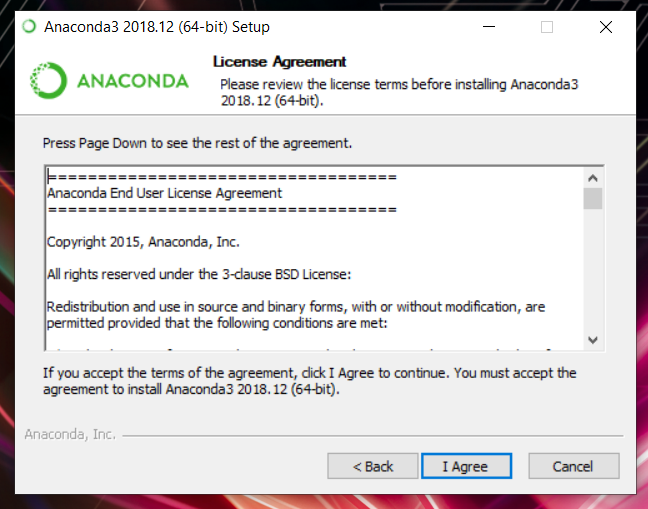
\includegraphics[width=3cm,height=3cm]{figures/felix/2.png}
        \caption{License}
        \label{awal}
        \end{figure}
    \item  Pilih untuk siapa aplikasi diinstal bisa just me dan juga bisa all users
     \begin{figure}[!htbp]
        \centering
        \includegraphics[width=3cm,height=3cm]{figures/felix/3.png}
        \caption{Proses}
        \label{awal}
        \end{figure}
    \item  Pilih lokasi instalasi
    \begin{figure}[!htbp]
        \centering
        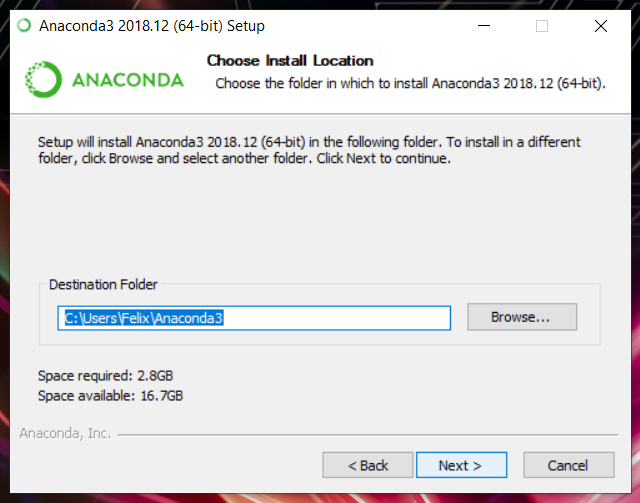
\includegraphics[width=3cm,height=3cm]{figures/felix/4.png}
        \caption{Proses}
        \label{awal}
        \end{figure}
    \item Pilih register anaconda karna add aconda environment tidak remomended
    \begin{figure}[!htbp]
        \centering
        \includegraphics[width=3cm,height=3cm]{figures/felix/5.png}
        \caption{Proses}
        \label{awal}
        \end{figure}
    \item Tunggu hingga selesai
    \begin{figure}[!htbp]
        \centering
        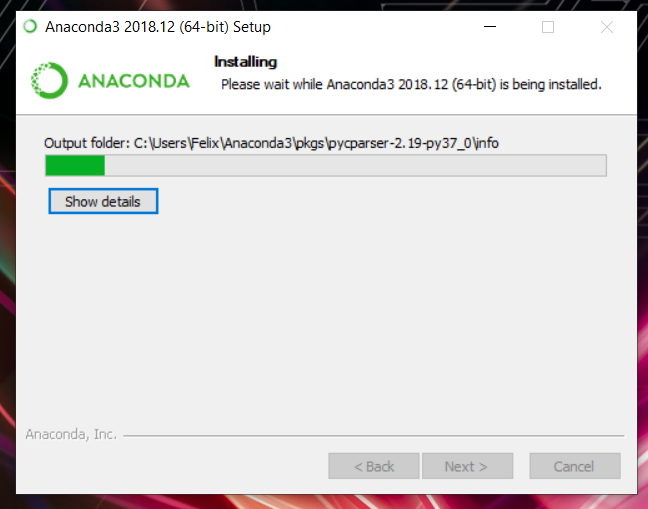
\includegraphics[width=3cm,height=3cm]{figures/felix/6.png}
        \caption{Proses}
        \label{awal}
        \end{figure}
    \item Klik skip
    \begin{figure}[!htbp]
        \centering
        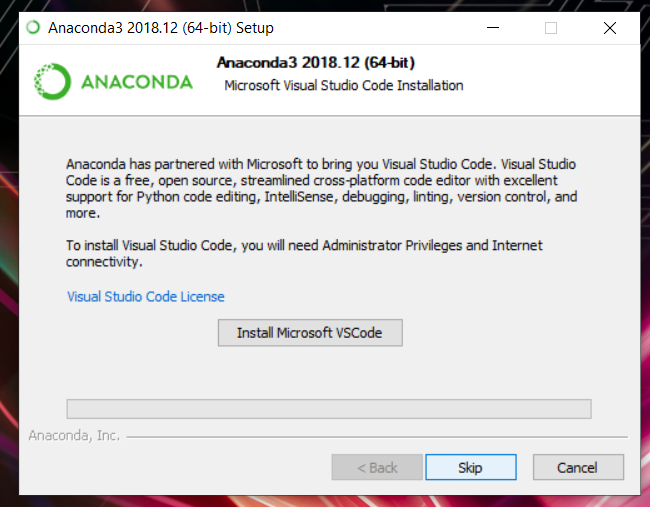
\includegraphics[width=3cm,height=3cm]{figures/felix/8.png}
        \caption{Proses}
        \label{awal}
        \end{figure}
    \item  Dan anaconda berhasil di install
    \begin{figure}[!htbp]
        \centering
        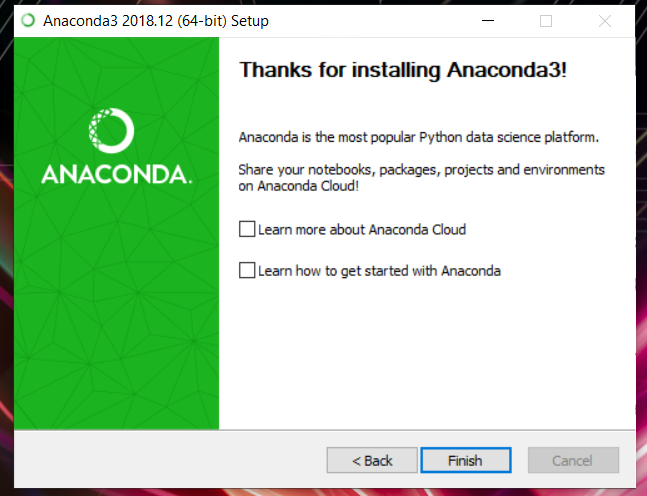
\includegraphics[width=3cm,height=3cm]{figures/felix/9.png}
        \caption{Proses}
        \label{awal}
        \end{figure}
\end{enumerate}
\subsection{Menggunakan Spyder}
setelah selesai menggunakan instalasi anaconda,  maka ada beberapa tool yang digunakan seperti spyder
\begin{figure}[!htbp]
        \centering
        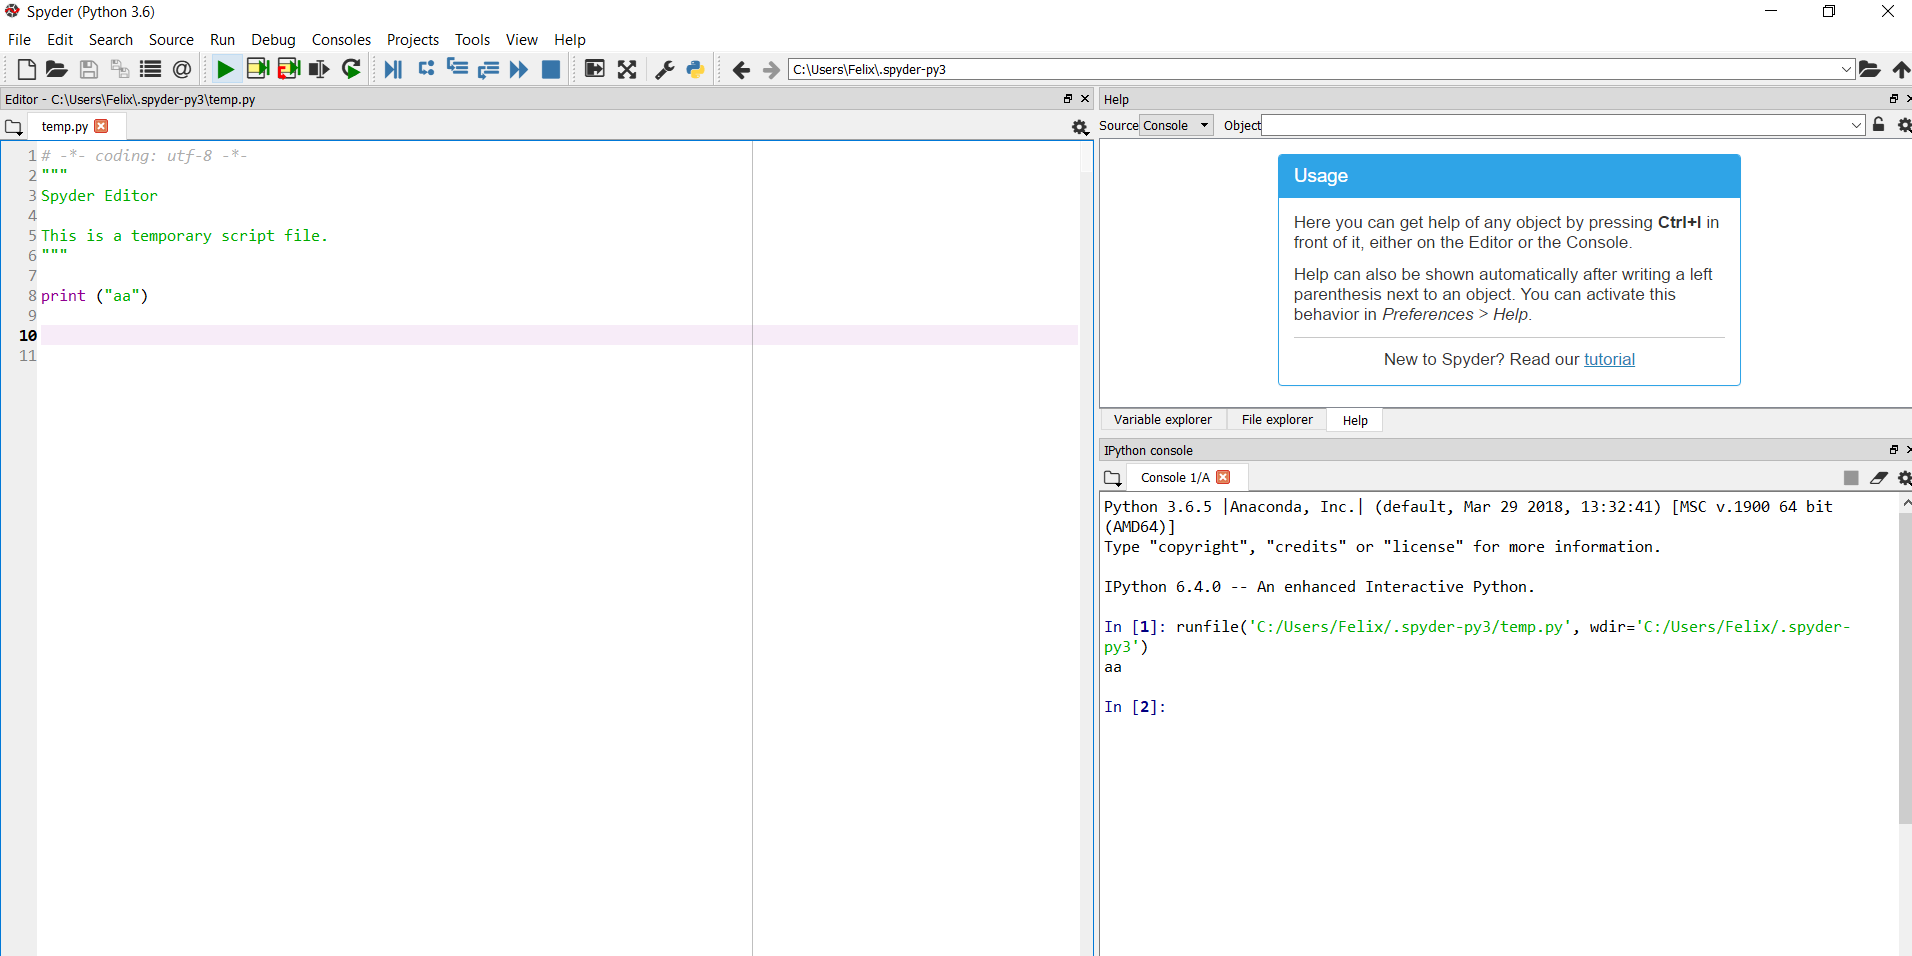
\includegraphics[width=3cm,height=3cm]{figures/felix/10.png}
        \caption{Proses}
        \label{awal}
        \end{figure}

Gambar tersebut menjelaskan tentang tampilan spyder dan mengeksekusi program aa